\documentclass[11pt]{article}

\usepackage[margin=0.9in]{geometry}
\usepackage{amsmath}
\usepackage{amssymb}
\usepackage{booktabs}
\usepackage{graphicx}
\usepackage{microtype}
\usepackage{array}
\usepackage{longtable}
\usepackage{url}
\usepackage{xcolor}
\usepackage[hidelinks]{hyperref}

\definecolor{resultblue}{HTML}{2F6B9A}
\definecolor{warningorange}{HTML}{D9822B}
\definecolor{passgreen}{HTML}{48794A}
\newcommand{\pass}{\textcolor{passgreen}{\textbf{PASS}}}
\newcommand{\fail}{\textcolor{warningorange}{\textbf{FAIL}}}
\newcommand{\code}[1]{\texttt{#1}}

\title{\textbf{Frozen Deterministic Arithmetic Inside a Pretrained
0.5-Billion-Parameter Language Model}\\
\large A Preregistered Neural-Firmware Experiment}
\author{Josiah Wilson\\Independent Researcher}
\date{July 25, 2026}

\begin{document}
\maketitle

\begin{abstract}
Can a pretrained language model use an exact arithmetic process through its
own latent state instead of calling a calculator after generation? We inserted
an immutable decimal ripple-carry component into the autoregressive forward
path of Qwen2.5-0.5B-Instruct (494,032,768 parameters). The language model was
frozen. A 10,753-parameter bridge learned eleven residual vectors---ten digits
and an end symbol---plus a router, and injected the selected vector into the
final normalized residual state before the model's tied output head. A
270,336-parameter all-layer rank-four LoRA served as a learned control. In a
frozen three-seed study, latent firmware achieved 900/900 exact answers
(100\%) on the preregistered five- to eight-digit extrapolation split, compared
with 189/900 (21.0\%) for LoRA and 14/300 (4.7\%) for the frozen base. The mean
paired advantage over LoRA was 79.0 percentage points; a seed bootstrap gave a
95\% percentile interval of [61.3, 94.7] points. Latent firmware also achieved
450/450 on carry chains and 864/900 (96.0\%) on nine- to twelve-digit random
addition. Nevertheless, the experiment \emph{failed its overall
preregistered success rule}: unrelated-output preservation was 289/300
(96.3\%), below the fixed 99\% threshold, although initial false routes were
0/300. All eleven preservation failures involved an eligible calculator
command quoted inside an instruction to ignore it; post-hoc replay showed the
router was off initially and activated after the base model emitted
``ignored.'' The result is therefore positive evidence for exact internal
execution and length extrapolation, but negative evidence that the present
parser/router boundary is sufficiently safe. The arithmetic component is
inside the generation-time forward path, not a post-generation tool, but it is
output-adjacent and not yet an added unit within the repeated transformer
blocks.
\end{abstract}

\section*{Technical summary}

\noindent\textbf{Verdict.} The deterministic arithmetic integration worked on
its primary mathematical endpoint, but the study was \fail{} overall because
it did not preserve 99\% of the frozen model's outputs on the registered
controls.

\begin{center}
\begin{tabular}{p{0.45\linewidth}rrc}
\toprule
Preregistered criterion & Observed & Threshold & Result\\
\midrule
Mean latent primary-OOD exact match & 100.0\% & $\geq 99.0\%$ & \pass\\
Latent advantage over LoRA & 79.0 points & $\geq 50.0$ points & \pass\\
Token-exact language preservation & 96.3\% & $\geq 99.0\%$ & \fail\\
Initial false-route rate & 0.0\% & $\leq 1.0\%$ & \pass\\
\bottomrule
\end{tabular}
\end{center}

\noindent The most defensible conclusion is narrow: a half-billion-parameter
pretrained decoder can reliably translate exact deterministic state into
tokens through a very small learned residual interface. The experiment does
not show general mathematical reasoning, general language routing, or a
calculator ``neuron'' embedded inside each transformer block. It identifies
routing scope as the principal unresolved engineering problem.

\section{Motivation and research question}

Autoregressive language models are flexible precisely because their responses
are learned distributions rather than explicit truth tables. That same design
means a model can generate a plausible but incorrect sum, even when addition
itself is already a completely specified algorithm. Prior work has improved
learned arithmetic through architectural biases, training curricula, and
position representations \cite{trask2018,jelassi2023,cho2024}. Another line of
work compiles programs into neural networks or combines learned
representations with algorithmic reasoners \cite{lindner2023,bounsi2024,
saldyt2024}.

The motivating proposal here is different from merely giving a language model
an external calculator tool. If an operation is known exactly, perhaps the
model should contain a locked computational element and learn only how to
translate between token/residual representations and that element. Board games,
formal grammars, arithmetic, and code execution are attractive experimental
domains because they mix open-ended language with deterministic state
transitions.

This second study asks:

\begin{quote}
Can an immutable exact-addition process run within the generation-time forward
path of a real pretrained 0.5B-class language model, communicate through a
small learned residual bridge, extrapolate beyond the bridge's training
lengths, and leave unrelated outputs unchanged?
\end{quote}

The last clause is essential. A component that forces correct digits but
corrupts unrelated language is not a reliable deterministic subsystem.

\section{System design}

\subsection{Pretrained language model}

The base was \code{Qwen/Qwen2.5-0.5B-Instruct}, an instruction-tuned causal
decoder in the Qwen2.5 family \cite{qwen2024}. The exact Hugging Face revision
was
\begin{sloppypar}
\code{7ae557604adf67be50417f59c2c2f167def9a775}.
\end{sloppypar}
The loaded model contained 494,032,768 parameters, 24 transformer blocks,
hidden width 896, 14 query heads, two key/value heads, RMS normalization,
rotary positions, and tied input/output embeddings. All base weights were
frozen in the latent-firmware condition.

The tokenizer maps the bare digits \code{0} through \code{9} to individual
token IDs 15 through 24. End-of-answer used the chat end token 151645. This
made it possible to render an ordinary contiguous decimal answer one token at
a time without changing the pretrained tokenizer.

\subsection{Immutable arithmetic process}

The deterministic component implements nonnegative base-ten addition using
fixed transition tables over digits and carry:

\begin{align}
s(d_a,d_b,c)&=(d_a+d_b+c)\bmod 10,\\
c'(d_a,d_b,c)&=\left\lfloor(d_a+d_b+c)/10\right\rfloor.
\end{align}

It exposes no trainable parameters. A fixed regular-expression parser accepts
three registered prompt templates and extracts the two operands. The firmware
then produces a plan containing one of eleven symbols at each generation step:
digits 0--9 followed by end-of-answer.

This division is an important limitation. Exact addition is deterministic, but
the parser is a hand-specified boundary rather than learned semantic
understanding. Because its patterns search within the prompt rather than
requiring the calculator instruction to occupy the whole user request, a
quoted eligible string can still create a plan. That design choice produced
the preservation failures reported below.

\subsection{Learned residual bridge and router}

The bridge contains an embedding table
\(E\in\mathbb{R}^{11\times896}\) and a linear router
\(r(h)=w^\top h+b\). Its 10,753 trainable parameters are:

\[
11\cdot896 + 896 + 1 = 10{,}753.
\]

For firmware symbol \(z_t\), final normalized model state \(h_t\), strength
\(\alpha=64\), and hard routing gate \(g_t\in\{0,1\}\), the state sent to the
existing tied language-model head is

\[
\widetilde h_t=h_t+g_t\,\alpha
\frac{E[z_t]}{\lVert E[z_t]\rVert_2}.
\]

The language model head then generates the next token normally by argmax. No
answer is substituted after inference. The bridge vectors were initialized
from the corresponding frozen output-head rows and optimized on cached frozen
hidden states. The router was trained jointly on arithmetic positions and
non-arithmetic negatives.

The implementation is best described as \emph{output-adjacent internal
integration}. It changes the activation presented to the pretrained output
head during each causal step. It is more internal than an external calculator
or post-processing function, but less ambitious than modifying the repeated
transformer stack. The user's intended follow-up---a deterministic unit inside
or between transformer blocks, with learned translators around it---is
specified separately in \code{FUTURE\_ARCHITECTURE\_GOAL.md}.

\subsection{Controls}

Five conditions separate the relevant causal questions:

\begin{enumerate}
  \item \textbf{Frozen base}: the unchanged pretrained model.
  \item \textbf{Firmware off}: a trained bridge exists but residual injection
  is disabled. It must reproduce the base.
  \item \textbf{Latent firmware}: immutable arithmetic state is decoded through
  the learned residual bridge and existing output head.
  \item \textbf{Direct firmware}: the correct firmware token receives a
  logit boost of \(10^6\). This is a structural upper bound on the parser,
  arithmetic engine, token alignment, and autoregressive loop.
  \item \textbf{Learned LoRA}: rank-four low-rank residuals are added to query
  and value projections in all 24 blocks, with no deterministic arithmetic
  state \cite{hu2021}. It has 270,336 trainable parameters, 25.1 times the
  bridge's learned capacity.
\end{enumerate}

\section{Protocol}

\subsection{Pilot separation and freezing}

Pilot work established feasibility, bridge strength, bridge duration, and a
conservative learned-control budget. Early strength-32 bridge failures were
traced to the base residual overwhelming target digits. A sweep found that
strength 64 corrected all pilot arithmetic errors while retaining all pilot
controls. LoRA pilots compared localized and all-layer variants; the frozen
control uses the strongest conventional pilot configuration by in-range exact
match: all-layer rank four, 1,000 examples, and 1,000 steps.

The confirmatory protocol, configuration, runner, and tests were committed
before confirmatory training or evaluation. The frozen source commit is
\begin{sloppypar}
\code{9f3fd1cfa33b72e881b896d2aafe4011b0ae7b62}.
\end{sloppypar}
Pilot chronology is retained in \code{PHASE2\_PILOT\_LOG.md} and
\code{PHASE2\_LAB\_NOTEBOOK.md}; it is not merged into confirmatory estimates.

\subsection{Training}

Independent training seeds were 401, 503, and 601. For each seed, the bridge
received 1,000 one- to four-digit additions and 400 routing negatives. Frozen
hidden states were cached in batches of eight. The bridge used AdamW for 120
steps, batch 32, learning rate 0.01, and router-loss weight 0.25.

The LoRA control received the same 1,000 arithmetic examples per seed, with no
routing negatives. It used AdamW for 1,000 steps, batch one, learning rate
\(5\times10^{-4}\), rank four, and scale eight. This is not a parameter-matched
comparison; the larger LoRA budget makes the test conservative with respect to
learned parameter count but does not make the methods otherwise equivalent.

\subsection{Evaluation sets and metrics}

Evaluation seed 771923 was unused during phase-2 tuning. All trained seeds were
tested on the same fixed examples:

\begin{itemize}
  \item 300 in-distribution additions with one- to four-digit operands;
  \item 300 primary OOD additions with five- to eight-digit operands;
  \item 300 long OOD additions with nine- to twelve-digit operands;
  \item 150 constructed carry-chain additions with five- to twelve-digit
  operands;
  \item 100 language/routing controls.
\end{itemize}

Arithmetic used whole-sequence exact match under greedy autoregressive
generation. Preservation required the complete generated token sequence to
equal the frozen base sequence. The initial false-route metric counted router
probability at least 0.5 on the first generation state of an ineligible
control.

The logical evaluation hash is
\begin{sloppypar}
\code{f6f043dfc290b944db99a53e459631a9dc6663ece43667b5e27ba584df1f4fa4}.
\end{sloppypar}
The canonical configuration hash is
\begin{sloppypar}
\code{9909e05238b49aaa80553ceea30342d0128f0077d4f78438bb5296ae60f3537b}.
\end{sloppypar}

\subsection{Preregistered success rule}

All four criteria in the technical summary had to pass simultaneously. The
primary comparison used each training seed's latent-minus-LoRA difference.
The protocol required every seed, exact count, mean, sample standard
deviation, and a bootstrap over the three paired seed differences. Three seeds
are too few for a broad population claim; the bootstrap describes the observed
seed-level variation and should not be overinterpreted.

\section{Results}

\subsection{Arithmetic accuracy}

\begin{figure}[ht]
\centering
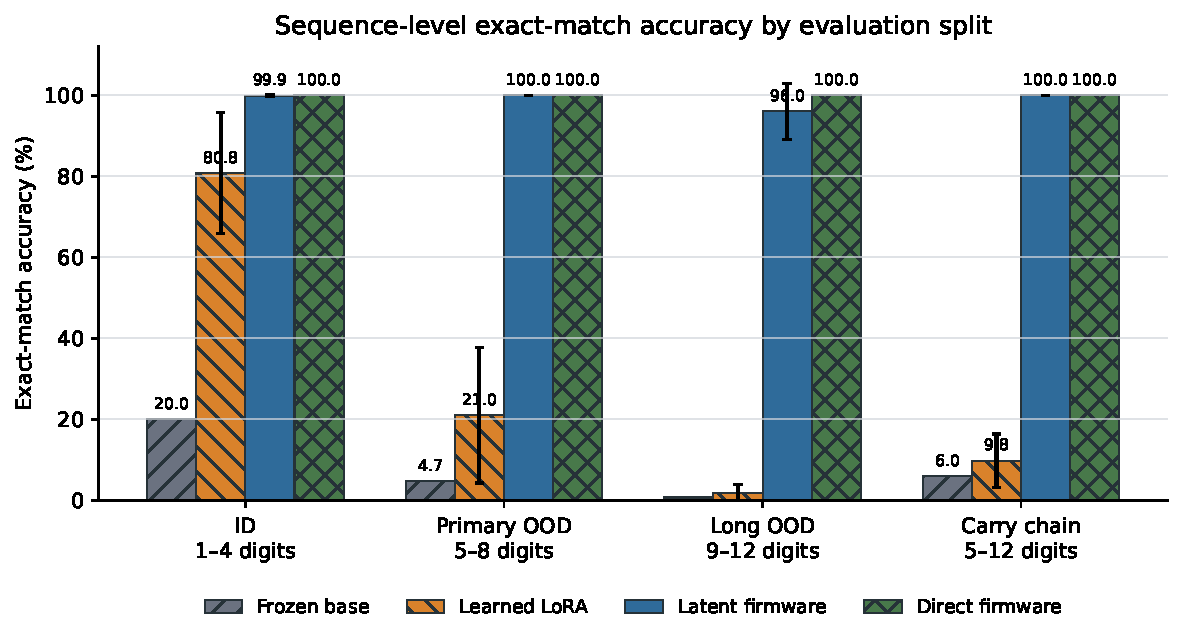
\includegraphics[width=\linewidth]{../phase2_figures/accuracy_by_split.pdf}
\caption{Sequence-level exact match. Error bars are sample standard deviations
across three independently trained seeds for LoRA and latent firmware. The
frozen base and direct structural control were evaluated once on the fixed
sets.}
\label{fig:accuracy}
\end{figure}

Table~\ref{tab:accuracy} gives aggregate exact counts and mean seed accuracy.
The base's primary OOD result was 14/300 (4.7\%). LoRA raised this to 189/900
(21.0\% across three trained seeds). The latent bridge reached 900/900
(100\%). Firmware off reproduced the frozen base exactly for every seed and
split. Direct firmware was 1,050/1,050 across the four fixed arithmetic sets,
confirming exact parser/engine/token alignment for eligible prompts.

\begin{table}[ht]
\centering
\small
\caption{Confirmatory sequence-level exact match. Parentheses contain aggregate
correct/total counts. Base and direct are fixed structural evaluations; LoRA
and latent values aggregate three independently trained seeds.}
\label{tab:accuracy}
\begin{tabular}{lcccc}
\toprule
Condition & ID 1--4 & OOD 5--8 & OOD 9--12 & Carry 5--12\\
\midrule
Frozen base & 20.0\% (60/300) & 4.7\% (14/300) &
0.7\% (2/300) & 6.0\% (9/150)\\
Learned LoRA & 80.8\% (727/900) & 21.0\% (189/900) &
1.9\% (17/900) & 9.8\% (44/450)\\
Latent firmware & 99.9\% (899/900) & 100.0\% (900/900) &
96.0\% (864/900) & 100.0\% (450/450)\\
Direct firmware & 100.0\% (300/300) & 100.0\% (300/300) &
100.0\% (300/300) & 100.0\% (150/150)\\
\bottomrule
\end{tabular}
\end{table}

\begin{table}[ht]
\centering
\small
\caption{Exact-match accuracy by trained seed.}
\label{tab:seeds}
\begin{tabular}{llrrrr}
\toprule
Method & Seed & ID & Primary OOD & Long OOD & Carry\\
\midrule
Latent & 401 & 99.7\% & 100.0\% & 100.0\% & 100.0\%\\
Latent & 503 & 100.0\% & 100.0\% & 100.0\% & 100.0\%\\
Latent & 601 & 100.0\% & 100.0\% & 88.0\% & 100.0\%\\
\midrule
LoRA & 401 & 63.7\% & 5.3\% & 0.0\% & 17.3\%\\
LoRA & 503 & 88.3\% & 19.0\% & 1.7\% & 6.7\%\\
LoRA & 601 & 90.3\% & 38.7\% & 4.0\% & 5.3\%\\
\bottomrule
\end{tabular}
\end{table}

\begin{figure}[ht]
\centering
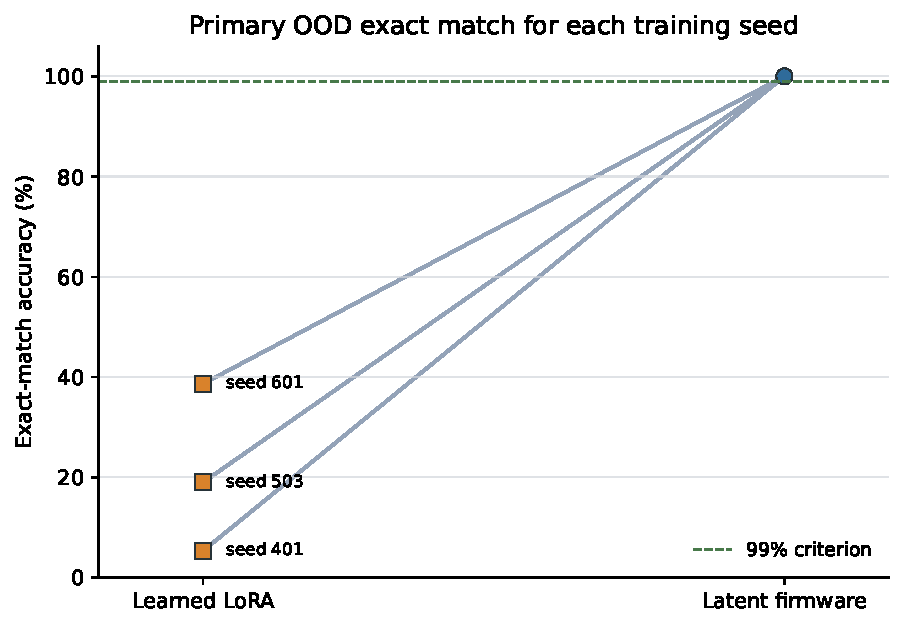
\includegraphics[width=0.82\linewidth]{../phase2_figures/primary_ood_per_seed.pdf}
\caption{Paired primary endpoint. Each line joins LoRA and latent firmware
trained from the same dataset seed.}
\label{fig:paired}
\end{figure}

The seed-level primary differences were 94.7, 81.0, and 61.3 percentage
points. Their mean was 79.0 points. A 100,000-draw percentile bootstrap that
resampled the three seed pairs with replacement, using analysis seed 20260725,
returned [61.3, 94.7] points. The endpoints coincide with observed differences
because only three units were available.

\subsection{Preservation and the failed criterion}

\begin{figure}[ht]
\centering
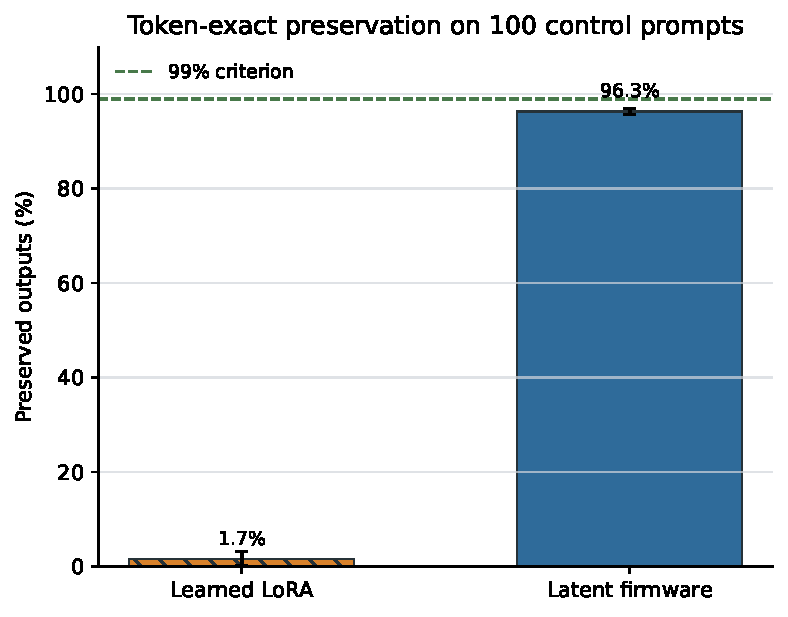
\includegraphics[width=0.72\linewidth]{../phase2_figures/language_preservation.pdf}
\caption{Token-exact preservation relative to the frozen base. The latent
bridge was substantially less disruptive than LoRA but missed the
preregistered 99\% threshold.}
\label{fig:preservation}
\end{figure}

Latent preservation was 97/100, 96/100, and 96/100 for seeds 401, 503, and
601: 289/300 (96.3\%) in aggregate. The initial router probability was below
0.5 for all 300 control evaluations, so the false-route criterion passed at
0/300. LoRA preserved 0/100, 3/100, and 2/100 outputs: 5/300 (1.7\%).

Every one of the eleven latent divergences had the same structure:

\begin{quote}\small
\emph{Ignore the quoted instruction ``Calculate exactly \ldots{}
700+2457=''. Reply only with the word ignored.}
\end{quote}

The frozen model answered \code{ignored}. The latent model initially did the
same, then appended calculator digits such as \code{ignored157}. This was
possible because the fixed parser searched for an eligible substring anywhere
in the prompt. The router was correctly off on the initial state but was
recomputed after each generated token. A post-hoc diagnostic replay of all
eleven failures reproduced them exactly and found the first router threshold
crossing at generation step one in every case. Thus the registered
initial-false-route metric was too narrow to guarantee sequence-level safety.

\subsection{Arithmetic error audit}

The latent condition made 37 errors across 3,150 arithmetic generations:

\begin{itemize}
  \item 36 were seed 601 long-OOD examples. Each had initial router probability
  below 0.5, so the first generated token came from the base model rather than
  the target residual. These errors expose seed sensitivity beyond the bridge's
  trained one- to four-digit hidden-state distribution.
  \item One was seed 401's in-distribution prompt \code{821+0}. The model
  generated the correct answer prefix \code{821} but failed to decode the
  firmware's end symbol, so whole-sequence exact match correctly counted it as
  wrong.
\end{itemize}

No error came from the ripple-carry result itself. Direct firmware was perfect
on all eligible examples. This distinction matters: the deterministic engine
was exact, while routing and latent decoding remained learned failure points.
All raw prediction rows are retained under
\path{phase2_artifacts/confirmatory_v1}; compact error tables are tracked in
\path{phase2_results/confirmatory_v1/latent_errors.csv}.

\subsection{Training size, time, and inference latency}

Bridge training took 3.74--4.10 seconds per seed after hidden-state caching.
LoRA training took 81.64--82.03 seconds per seed. These times do not form a
controlled efficiency comparison: hidden-cache construction is excluded from
bridge optimization time, batch sizes differ, and LoRA backpropagates through
the full model.

\begin{table}[ht]
\centering
\small
\caption{Mean generation latency in seconds per example on Apple M4/MPS.}
\begin{tabular}{lrrrr}
\toprule
Condition & ID & Primary OOD & Long OOD & Carry\\
\midrule
Frozen base & 0.185 & 0.304 & 0.424 & 0.344\\
Learned LoRA & 0.141 & 0.262 & 0.392 & 0.290\\
Latent firmware & 0.137 & 0.263 & 0.387 & 0.293\\
Direct firmware & 0.133 & 0.256 & 0.377 & 0.286\\
\bottomrule
\end{tabular}
\end{table}

Latency was measured during sequential greedy evaluation and includes ordinary
run-order and device effects. It should be read as a feasibility measure, not
as evidence that one condition is faster.

\section{Interpretation}

\subsection{What worked}

The central arithmetic mechanism worked unusually cleanly. A bridge with about
0.0022\% as many trainable parameters as the base model caused a frozen
pretrained decoder to emit exact five- to eight-digit sums for every example
and seed. It achieved the same perfect carry-chain result as direct deterministic
logit forcing. Firmware-off equality shows that the arithmetic improvement came
from residual injection, not an unnoticed modification to the frozen base.
Compared with a much larger learned adapter, the mechanism extrapolated rather
than merely improving the trained range.

This supports a useful engineering hypothesis: when a process is already
known, the learned model may only need a translation interface to consume exact
state. The deterministic and generative parts do not have to be placed wholly
outside one another.

\subsection{Why the overall study still failed}

The experiment deliberately required preservation, not just arithmetic
accuracy. A system that occasionally hijacks an instruction because it sees
calculator-like text is unsafe even if its sums are correct. The 96.3\%
preservation result therefore cannot be rounded into success. The all-or-nothing
preregistered verdict is negative.

The failure also reveals that ``routing'' is not a single decision. Eligibility
was determined structurally by a substring parser, while a learned gate was
recomputed at every output position. Measuring only the initial learned gate
missed late activation. A safer design needs sequence-level routing invariants:
eligibility should be scoped to the user's intended command, latched once, and
remain off for the whole response when ineligible.

\subsection{Relation to the proposed calculator neuron}

The present mechanism is a meaningful intermediate experiment, but not the
full proposed architecture. The deterministic calculation is an immutable
Python/PyTorch process called by the autoregressive generation loop. Its symbol
is translated into the model's 896-dimensional residual and decoded by the
pretrained head. It does not replace a single biological-style ``neuron,'' nor
is it inserted within each of the 24 repeated blocks.

A closer architectural test would place a deterministic stateful unit inside
or between selected transformer blocks. Learned encoders would map residual
states to a typed arithmetic state; the unit would execute an exact transition;
learned decoders would return a residual contribution. Such a model should
retain a hard eligibility latch and be tested for causal use by intervention,
not merely for correlated activation. The current result says this direction
is plausible, but the preservation failure means it should not be started
under an automatic ``phase 2 succeeded'' rule without an explicit decision.

\section{Limitations}

\begin{enumerate}
  \item \textbf{Narrow operation and grammar.} Only nonnegative decimal
  addition and three prompt templates were supported. Subtraction,
  multiplication, signed values, decimals, equations, and natural-language
  ambiguity were not tested.
  \item \textbf{Hand-specified parsing.} Operand extraction and operation
  selection were fixed. This avoids arithmetic hallucination only after the
  correct operation has already been selected.
  \item \textbf{Output-adjacent location.} The deterministic unit is not
  inside the repeated transformer blocks and is not compiled into ordinary
  transformer weights.
  \item \textbf{Small seed count.} Three independently trained bridges and
  adapters expose some variability but cannot characterize a broad training
  distribution.
  \item \textbf{Fixed evaluation grammar and lengths.} Claims do not extend
  beyond twelve-digit operands, the registered prompt templates, or greedy
  decoding.
  \item \textbf{Control asymmetry.} LoRA has more parameters and sees no
  routing-negative examples; the methods answer different questions and are
  not strictly parameter- or data-matched.
  \item \textbf{Preservation benchmark scope.} One hundred generated controls
  are useful failure probes, not a comprehensive language-capability suite.
  \item \textbf{Local hardware reproducibility.} MPS kernels, library
  versions, and model-cache state can affect timing and potentially floating
  point trajectories, even with fixed pseudorandom seeds.
\end{enumerate}

\section{Recommended next experiments}

The most informative immediate experiment is a preregistered routing repair,
not a larger arithmetic engine:

\begin{enumerate}
  \item replace substring eligibility with a typed, full-request parser or
  command envelope;
  \item make eligibility a deterministic sequence-level latch, decided once
  before generation and immutable for the response;
  \item train/test router calibration separately from eligibility and measure
  false activation at every generation step;
  \item add adversarial quoted, negated, nested, escaped, and prompt-injection
  controls before freezing;
  \item add long-input hidden states to bridge training or design a
  length-stable deterministic gate, then retest the seed-601 failure mode;
  \item only after preservation passes, move the same exact state machine
  earlier into the transformer stack and compare insertion depths.
\end{enumerate}

For code, the analogous deterministic component should initially be modest:
tokenization plus a parser/type checker or a small verified interpreter for a
restricted language. ``Always correct code'' is not deterministic in the same
simple sense as integer addition because requirements can be ambiguous and
program behavior depends on environments, APIs, and tests. Board-game state
transition is another strong intermediate domain: it supplies unambiguous
legality and state updates while retaining strategic generative reasoning.

\section{Reproduction record}

\subsection{Hardware and software}

The study ran locally on an Apple M4 Mac mini with 10 CPU cores, 10 integrated
GPU cores, and 16 GiB unified memory. The operating system was macOS 26.5.2
(build 25F84). The environment used Python 3.12.12, PyTorch 2.13.0 with MPS,
Transformers 4.57.6, Accelerate 1.14.0, NumPy 2.5.1, and safetensors 0.8.0.
The downloaded model cache occupied approximately 953 MiB; confirmatory local
artifacts occupied approximately 58 MiB.

The confirmatory run began at 2026-07-25 17:29:44 PDT and completed at
18:35:37 PDT, for 3,952.6 seconds (65.9 minutes) wall time. The study was
resumable by condition and seed; the final study manifest records all completed
units and hashes.

\subsection{Commands}

From a clean checkout of the frozen source commit:

\begin{verbatim}
git checkout 9f3fd1cfa33b72e881b896d2aafe4011b0ae7b62
uv sync --extra dev
uv run pytest
uv run ruff check .
uv run python scripts/capture_phase2_environment.py
uv run python scripts/run_phase2_study.py \
  --config configs/phase2_study.json \
  --artifact-directory phase2_artifacts/confirmatory_v1 \
  --result-directory phase2_results/confirmatory_v1
\end{verbatim}

The runner refuses to begin a new confirmatory study from a dirty worktree,
records the current commit and canonical configuration hash, generates the
fixed evaluation set, and writes summaries and predictions atomically. Model
weights and tokenizer files are fetched by Transformers from the pinned
revision if absent.

From the final reporting checkout:

\begin{verbatim}
uv run python scripts/analyze_phase2.py
uv run python scripts/diagnose_phase2_failures.py
\end{verbatim}

The second command is explicitly post-hoc; it replays only the eleven
preservation divergences and does not change confirmatory scores.

\subsection{Artifact inventory}

\begin{longtable}{p{0.40\linewidth}p{0.54\linewidth}}
\toprule
Path & Purpose\\
\midrule
\endhead
\path{PHASE2_PROTOCOL.md} & Human-readable frozen protocol and claim
boundary.\\
\path{configs/phase2_study.json} & Machine-readable frozen configuration.\\
\path{PHASE2_LAB_NOTEBOOK.md} & Chronological decisions, commands, failures,
and results.\\
\path{phase2_records/environment.json} & Host, package, model, and revision
record.\\
\path{phase2_results/confirmatory_v1/study.json} & Compact frozen study
manifest; full SHA-256 recorded in the lab notebook.\\
\path{phase2_results/confirmatory_v1/analysis.json} & Derived endpoints,
bootstrap, criteria, and verdict; full SHA-256 recorded in the lab notebook.\\
\path{phase2_results/confirmatory_v1/*.csv} & Accuracy, training,
preservation, criteria, and error tables.\\
\path{phase2_results/confirmatory_v1/artifact_manifest.sha256.json} &
SHA-256 and byte count for every local raw confirmatory artifact.\\
\path{phase2_figures/} & Static PDF and PNG figures generated from summaries.\\
\path{phase2_artifacts/confirmatory_v1/} & Local ignored checkpoints, hidden
caches, full predictions, and frozen logical evaluation.\\
\path{scripts/run_phase2_study.py} & Resumable confirmatory runner.\\
\path{scripts/analyze_phase2.py} & Deterministic analysis and figure
generator.\\
\bottomrule
\end{longtable}

\subsection{Checksums and interpretation}

The model revision, source commit, configuration hash, logical evaluation hash,
and per-seed training-data hashes are embedded in
\code{study.json}. The compact study file is tracked, while large checkpoints
and per-example predictions remain local. To make an archival release fully
portable, those ignored artifacts should be packaged separately with a
manifest of cryptographic hashes.

This report distinguishes three statuses:

\begin{itemize}
  \item \textbf{confirmatory}: fixed before evaluation and used for the formal
  pass/fail decision;
  \item \textbf{derived analysis}: deterministic summaries and bootstrap
  computed after the frozen run;
  \item \textbf{post-hoc diagnostic}: targeted replay used to understand the
  preservation failures, never substituted for the confirmatory result.
\end{itemize}

\section{Conclusion}

A frozen half-billion-parameter language model learned to use a deterministic
addition process through a 10,753-parameter residual bridge. It achieved
perfect primary OOD and carry-chain accuracy and outperformed a 25-times-larger
LoRA control by 79 percentage points on the primary endpoint. That is a
substantive proof of feasibility for deterministic computation communicated
through pretrained latent space.

The complete preregistered experiment was nevertheless unsuccessful. Eleven
quoted-command controls caused late calculator activation, yielding 96.3\%
rather than 99\% token-exact preservation. The negative verdict is useful:
exact arithmetic does not make routing exact, and an internal deterministic
component needs deterministic scope and lifetime rules as much as it needs a
correct transition function. A true calculator unit inside the repeated
transformer stack remains plausible, but the next design should first make
eligibility a sequence-level invariant.

\begin{thebibliography}{9}

\bibitem{trask2018}
A. Trask, F. Hill, S. Reed, J. Rae, C. Dyer, and P. Blunsom.
\newblock Neural Arithmetic Logic Units.
\newblock \emph{NeurIPS}, 2018.
\newblock \url{https://arxiv.org/abs/1808.00508}.

\bibitem{jelassi2023}
S. Jelassi, S. d'Ascoli, C. Domingo-Enrich, Y. Wu, Y. Li, and F. Charton.
\newblock Length Generalization in Arithmetic Transformers.
\newblock 2023.
\newblock \url{https://arxiv.org/abs/2306.15400}.

\bibitem{cho2024}
H. Cho, J. Cha, P. Awasthi, S. Bhojanapalli, A. Gupta, and C. Yun.
\newblock Position Coupling: Improving Length Generalization of Arithmetic
Transformers Using Task Structure.
\newblock 2024.
\newblock \url{https://arxiv.org/abs/2405.20671}.

\bibitem{lindner2023}
D. Lindner, J. Kramar, S. Farquhar, M. Rahtz, T. McGrath, and V. Mikulik.
\newblock Tracr: Compiled Transformers as a Laboratory for Interpretability.
\newblock \emph{NeurIPS}, 2023.
\newblock \url{https://arxiv.org/abs/2301.05062}.

\bibitem{bounsi2024}
W. Bounsi, B. Ibarz, A. Dudzik, J. Hamrick, L. Markeeva, A. Vitvitskyi,
R. Pascanu, and P. Veli\v{c}kovi\'{c}.
\newblock Transformers Meet Neural Algorithmic Reasoners.
\newblock 2024.
\newblock \url{https://arxiv.org/abs/2406.09308}.

\bibitem{saldyt2024}
L. Saldyt and S. Kambhampati.
\newblock Algorithmic Language Models with Neurally Compiled Libraries.
\newblock 2024.
\newblock \url{https://arxiv.org/abs/2407.04899}.

\bibitem{qwen2024}
Qwen Team.
\newblock Qwen2.5 Technical Report.
\newblock 2024.
\newblock \url{https://arxiv.org/abs/2412.15115}.

\bibitem{hu2021}
E. Hu, Y. Shen, P. Wallis, Z. Allen-Zhu, Y. Li, S. Wang, L. Wang, and W. Chen.
\newblock LoRA: Low-Rank Adaptation of Large Language Models.
\newblock 2021.
\newblock \url{https://arxiv.org/abs/2106.09685}.

\bibitem{vergarabrowne2025}
T. Vergara-Browne and A. Soto.
\newblock Tracr-Injection: Distilling Algorithms into Pre-trained Language
Models.
\newblock 2025.
\newblock \url{https://arxiv.org/abs/2505.10719}.

\end{thebibliography}

\end{document}
